%
% Tallinn University of Technology - bachelor, master thesis template for LaTeX
%
% Public Version 1.1
% 2019 Adjusted by Frank Korving for his Bachelor Thesis, with contributions from Sander Arnus
%
% Public version 1.0
% 2010 - 2013 Thijs Nugteren and Joos Buijs for Master Thesis
%
% THIS IS THE MAIN FILE (i.e. compile this file, compiling the others directly won't work)
%
\documentclass[12pt, a4paper]{report}

% all the other includes etc. are done in the thesis.sty file.
\usepackage{thesis}
\usepackage{biblatex}

%
% These commands need to be defined in order to produce a correct and personalized document
%
\newcommand{\doctitle}{Web system for self build car dashboard}
\newcommand{\docsubtitle}{Distributed Systems project}

\newcommand{\me}{Tavo Annus}
\newcommand{\studentcode}{186060IAIB}
\newcommand{\university}{TALLINN UNIVERSITY OF TECHNOLOGY}
\newcommand{\school}{School of Information Technologies}
\newcommand{\department}{Your Department}

\newcommand{\supervisor}{Andres Käver}
\newcommand{\supervisortitle}{BsC}
\newcommand{\keywords}{Important, comma, separated, keywords, applicable, to, your, thesis}
\newcommand{\version}{0.1 version}
\newcommand{\monthYear}{Month Year}
\newcommand{\Year}{2021}
\newcommand{\signatureDate}{Month Day, Year}

\author{\meone \metwo}

%
% PDF settings
%
\hypersetup
{
    pdfauthor={\me},
pdfsubject={\doctitle},
pdfkeywords={\keywords}
}

\begin{document}
    \pagenumbering{roman}
    \begin{titlepage}
    \headheight = 57pt
    \footskip = 5pt
    \headsep = 0pt

    \centering
    \textsc{\begin{Large}
                \university\\
    \end{Large} }
    \school\\
    \department\\

    \vspace*{7 cm}

    \begin{center}

        \me \quad \studentcode\\
        \begin{Large}
            \textsc{\textbf{\doctitle}}\\
        \end{Large}
        \docsubtitle\\
    \end{center}

    \begin{flushright}
        \textbf{Supervisor}\\ \supervisor\\\supervisortitle\\
    \end{flushright}

    \vfill

    Tallinn \Year
\end{titlepage}

    \normalsize

    \chapter*{\centerline{Author's declaration of originality}}\label{ch:declaration}
    \hfill \\
I hereby certify that I am the sole author of this thesis. All the used materials, references
to the literature and the work of others have been referred to. This thesis has not been
presented for examination anywhere else.

\vskip1in
\begin{flushleft}
    \begin{tabular}{p{2.0cm}p{6.0cm}p{4.0cm}}
        Author: & \me & ......................................\\
        && \hfill(signature)\\
        Date: & \signatureDate &\\
        \\
        \\

% Uncomment the following to add supervisor declaration
%  \multicolumn{3}{l}{The thesis adheres to all specified requirements}\\
%  \hfill \\
%  Supervisor: & \supervisor & ......................................\\
%  && \hfill(signature)\\
%  Date: & \signatureDate &\\


    \end{tabular}
\end{flushleft}

%    \chapter*{\centerline{Annotatsioon}}\label{ch:abstract-eesti}
%    Lõputöö on kirjutatud ... keeles ning sisaldab teksti ... leheküljel, ... peatükki, ... joonist, ... tabelit.
%    \pagebreak
%
%    \chapter*{\centerline{Abstract}}\label{ch:abstract}
%    The thesis is in ... and contains ... pages of text, ... chapters, ... figures, ... tables.
%    \pagebreak

    \chapter*{\centerline{List of abbreviations and terms}}\label{ch:terms}
    \begin{longtable}{p{3cm}p{10cm}}
    API&Application Programming Interface\\
    ERD&Entity Relations Diagram\\
    CAN&Controller Area Network\\
\end{longtable}
\addtocounter{table}{-1}
    \pagebreak

    \phantomsection
    \setcounter{tocdepth}{2}    % Sets maximum depth of Table Of Contents
    \renewcommand{\contentsname}{Table of Contents}
    \tableofcontents

%    \clearpage \phantomsection
%    \setcounter{figure}{0}
%    \addcontentsline{toc}{chapter}{\listfigurename}
%    \listoffigures
%
%    \clearpage \phantomsection
%    \addcontentsline{toc}{chapter}{\listtablename}
%    \listoftables

    \chapter{Introduction}\label{ch:introduction}
    \onehalfspacing
    \setcounter{page}{0}
    \pagenumbering{arabic}   %from here on, start the 'real' page numbering, from 1, with normal digits
    There are many free Apps for both PC and Android to diagnose your car via OBD2 port.
These Apps give access to data such as fault codes, current rpm, oil temperature and many more.
Since older cars don't have fancy touch screens it would make sense to have some app running and reading this data to show out on screen.

To have more general statistics for a driver it would make sense to sync them up to some database so that you could access the data also outside your car.
This would also give the possibility to see stats containing many cars and compare different car marks / models stats to one another.


\section{Project scope}\label{sec:project-scope}
The scope of this project is to build web application and database system capable of storing and querying data from multiple users at once.
Building an app capable of reading desired data from a car is not in the scope of this project and will be done at a later time.

\textbf{Must haves:}
\begin{itemize}
    \item ERD schema.
    \item Controllers for desired CRUD operations with entities.
\end{itemize}

    \chapter{ERD schema}\label{ch:erd_schema}
    Application ERD schema is shown on Figure
\ref{fig:erd-schema}

\begin{figure}[h]
    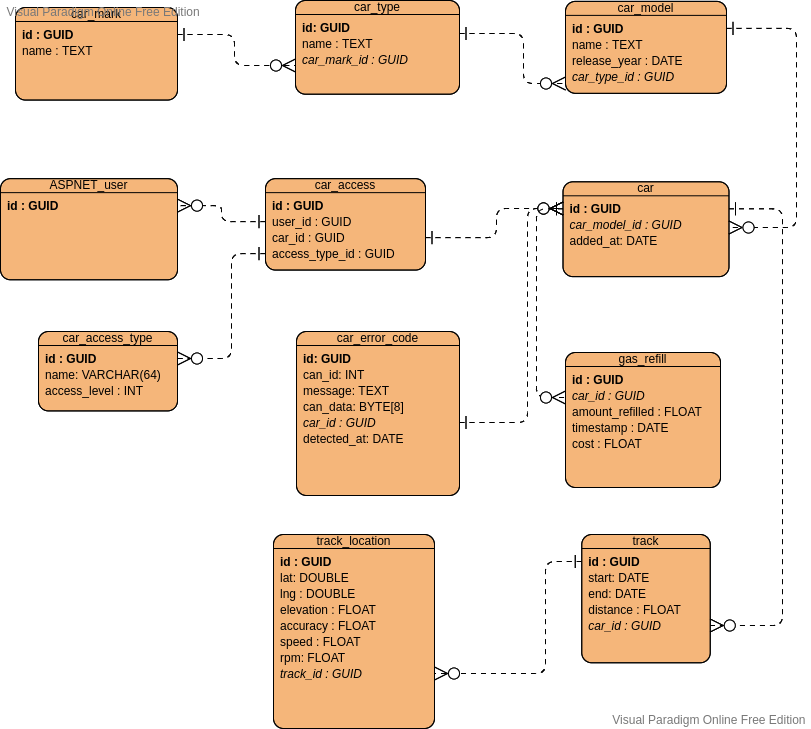
\includegraphics[width=\textwidth]{figures/erd_schema}
    \caption{ERD schema}
    \label{fig:erd-schema}
\end{figure}

ASP NET user part and user roles part is subject to change as we are covering them later in the lectures.

    \chapter{Second Chapter}\label{ch:second_chapter}
    One of the best resources for \LaTeX basics, and advanced constructs, is the \LaTeX wikibook\footnote{To be found at~\url{http://en.wikibooks.org/wiki/LaTeX/}}. Of course fellow students, colleagues and a good internet search using your favorite search engine can do wonders if you're stuck.

    \chapter{Summary}\label{ch:summary}
    \input{chapters/summary.tex}

    \pagebreak
    \phantomsection
    \addcontentsline{toc}{chapter}{Bibliography}
    \printbibliography

    \pagebreak
    \phantomsection
    \appendix
    \addcontentsline{toc}{chapter}{Appendices}
    \chapter*{Appendices}
    \renewcommand{\thechapter}{\arabic{chapter}}

    \addcontentsline{toc}{chapter}{Appendix 1 - Something}\label{chapter:appendix-one}
    {\let\clearpage\relax\chapter*{Appendix 1 - Something}}
    \begin{lstlisting}[frame=single, basicstyle=\small]
<!DOCTYPE html>
<html>
<body>

<h1>Example Title</h1>

<p>Some text here</p>

</body>
</html>
\end{lstlisting}

\end{document}